\section{Results}

\subsection{packages used (in methods)}

ade4 (1.7-22) for the computation of the Foucart Correspondence Analysis, ggplot2 (3.5.1) for the data visualization part, bipartite (2.19)

\subsection{Evaluate reconstruction and optimum research (C'est en double, il faut fusionner avec celui des methodes}

The efficiency of the Correspondence Analysis to recover the latent traits in the single network case has been well-documented by Lisa Nicvert. The goal here is to validate the multinetwork case, using Foucart's analysis.

In this section, we aim to evaluate the impact of the simulation parameters on the recovery of the latent traits within a series of networks. We performed 6 experiments to assess the effect of different factors:
\begin{itemize}
    \item the number of sampled interactions
    \item the number of sampled locations
    \item the environmental tolerance of the species
    \item the crossed impact of the size of the environmental niche and the number of sampled locations
    \item the weight given to trait matching in comparison to the mean-field effect
    \item the ratio between the traits 1 and 2 and finally the trait tolerance
\end{itemize}







\subsection{make a small intro!}

The performance was assessed by computing the mean correlation between trait one and the first axis position and similarly for the second trait and axis.



\subsubsection{Effect of the number of interactions ($n_{inter\_tot}$)}

\begin{figure}[H]
    \centering
    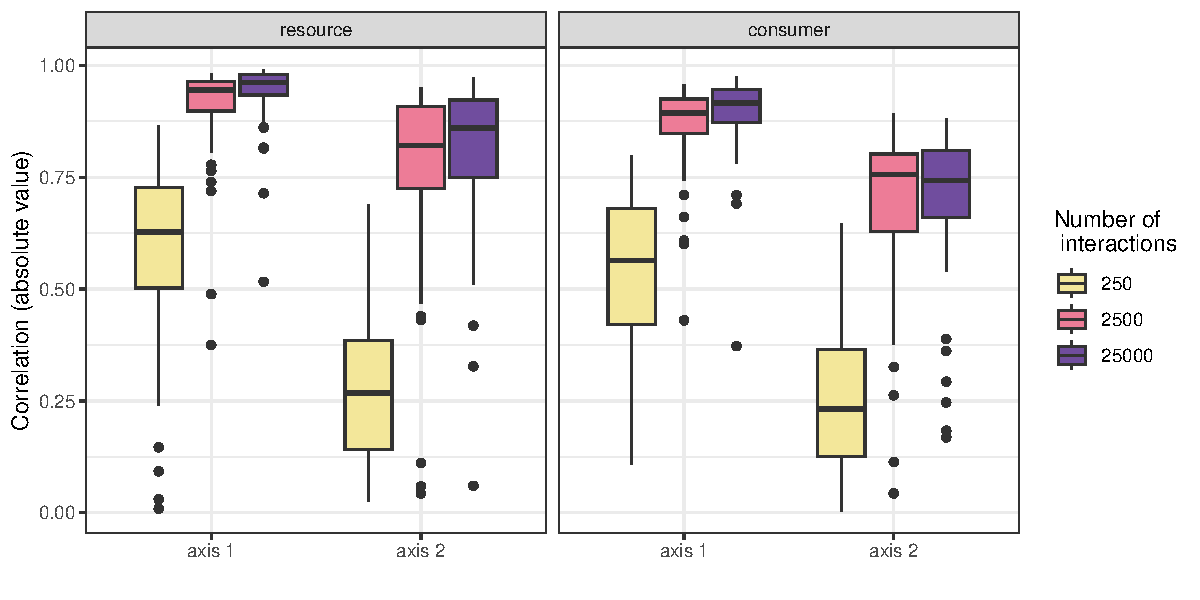
\includegraphics[width=0.75\linewidth]{FIGURES/ninter.pdf}
    \caption{Evaluation of the reconstruction of the trait depending on the total number of interactions observed (50 consumer species, 50 resource species, $n_{frame} = 5$, $\delta =  0.2$, $trait\_ratio = 0.7$, $\mu_{tol\_env} = 0.5$ and $\mu_{tol\_trait} = 0.1$)}
    \label{fig:ninter}
\end{figure}

The recovery of the traits increases with the number of interactions sampled across all the networks. Specifically, trait recovery is significantly higher when there is an equivalent of one observation per potential interaction. With ten times more observation, the improvement is marginal.

\subsubsection{Joint influence of the number of sampled locations and the environmental tolerance ($n_{frame} \times \mu_{tol\_env}$)}

\begin{figure}[H]
    \centering
    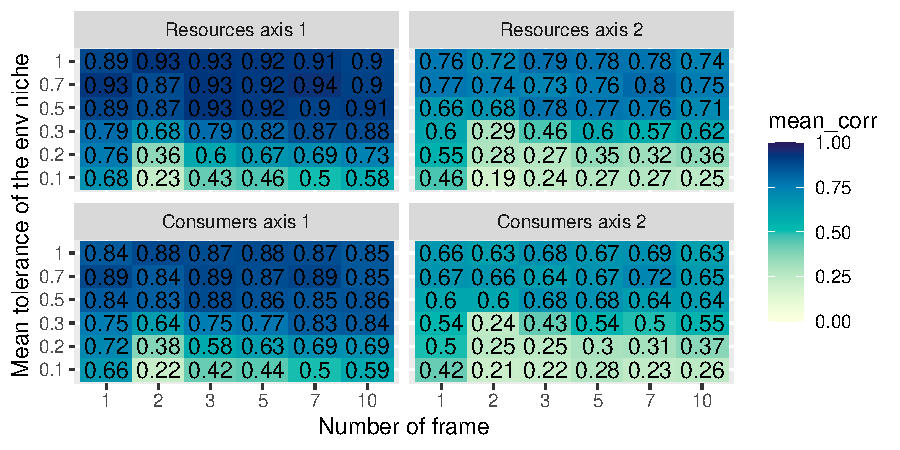
\includegraphics[width=0.75\linewidth]{FIGURES/frame_env.pdf}
    \caption{Evaluation of the reconstruction of the trait depending on the crossed effect of the number of sites and the environmental tolerance (50 consumer species, 50 resource species, $n_{inter\_tot} = 2500$, $\delta =  0.2$, $trait\_ratio = 0.7$ and $\mu_{tol\_trait} = 0.1$)}
    \label{fig:frame_env}
\end{figure}

The trait recovery significantly decreases when the number of sampled locations increases from one to two and for the low environmental tolerance values ($\mu_{tol\_env} < 0.7$). However, as the number of sampled sites continues to increase, trait recovery improves and matches the recovery observed in a single sampled site. Also, the trait recovery improves with higher environmental tolerance of the niche. When the mean environmental tolerance is $0.5$ or higher, the number of sampled sites no longer has a significant impact on the trait recovery.



\subsubsection{Effect of the weight given to trait matching ($\delta$)}

\begin{figure}[H]
    \centering
    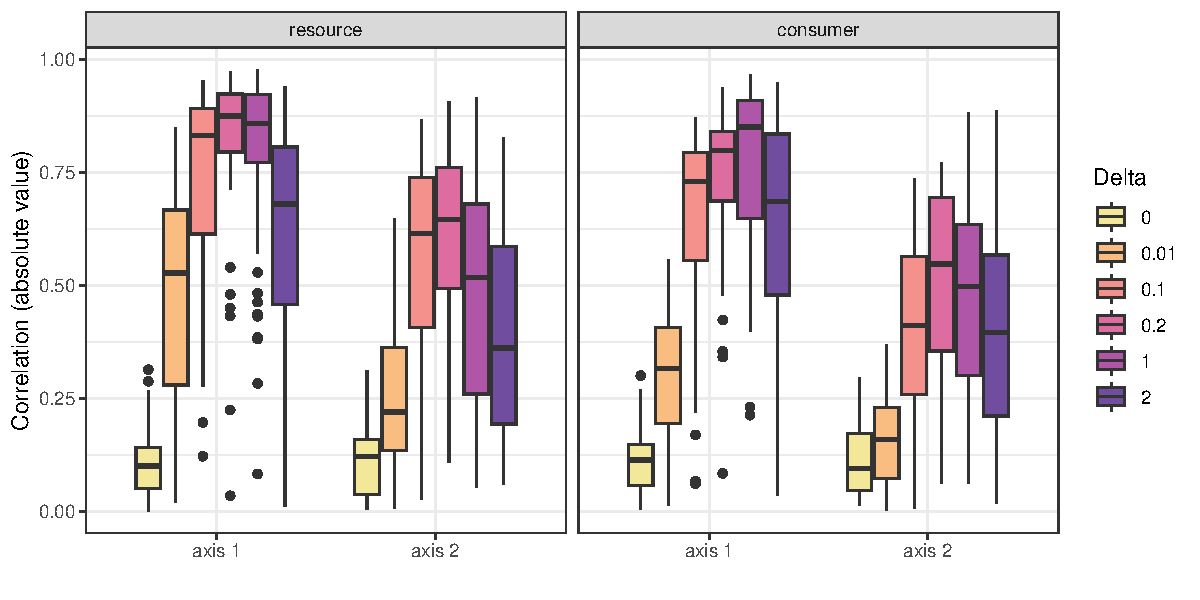
\includegraphics[width=0.75\linewidth]{FIGURES/delta.pdf}
    \caption{Evaluation of the reconstruction of the trait depending on the weight given to trait matching (delta) (50 consumer species, 50 resource species, $n_{inter\_tot} = 2500$, $n_{frame} = 5$,$trait\_ratio = 0.7$, $\mu_{tol\_env} = 0.5$ and $\mu_{tol\_trait} = 0.1$)}
    \label{fig:delta}
\end{figure}

Trait recovery increases with the weight given to trait matching ($\delta$) up to $\delta = 0.2$ after which it decreases when the trait matching is too important ($\delta = 2).$



\subsubsection{Effect of the relative weight given to the traits ($trait\_ratio$)}

\begin{figure}[H]
    \centering
    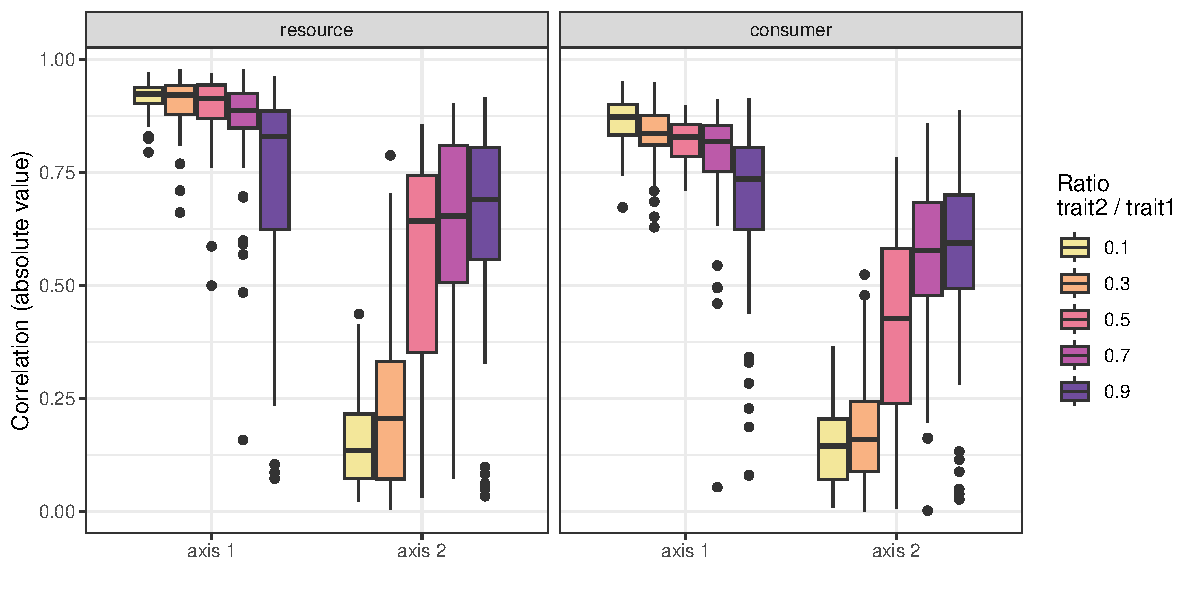
\includegraphics[width=0.75\linewidth]{FIGURES/ratio.pdf}
    \caption{Evaluation of the reconstruction of the trait depending on the ratio between the first and the second trait (50 consumer species, 50 resource species, $n_{inter\_tot} = 2500$, $n_{frame} = 5$, $\delta =  0.2$, $\mu_{tol\_env} = 0.5$ and $\mu_{tol\_trait} = 0.1$)}
    \label{fig:trait_ratio}
\end{figure}

When most of the weight is given to the first trait, the correlation between the first axis and the first trait is the highest, while the correlation between the second axis and the second trait is the lowest. As the weight given to the second trait increases, the correlation between the first axis and the first trait decreases, and the correlation between the second trait and the second axis increases.


\subsubsection{Effect of the trait tolerance ($\mu_{tol\_trait}$)}

\begin{figure}[H]
    \centering
    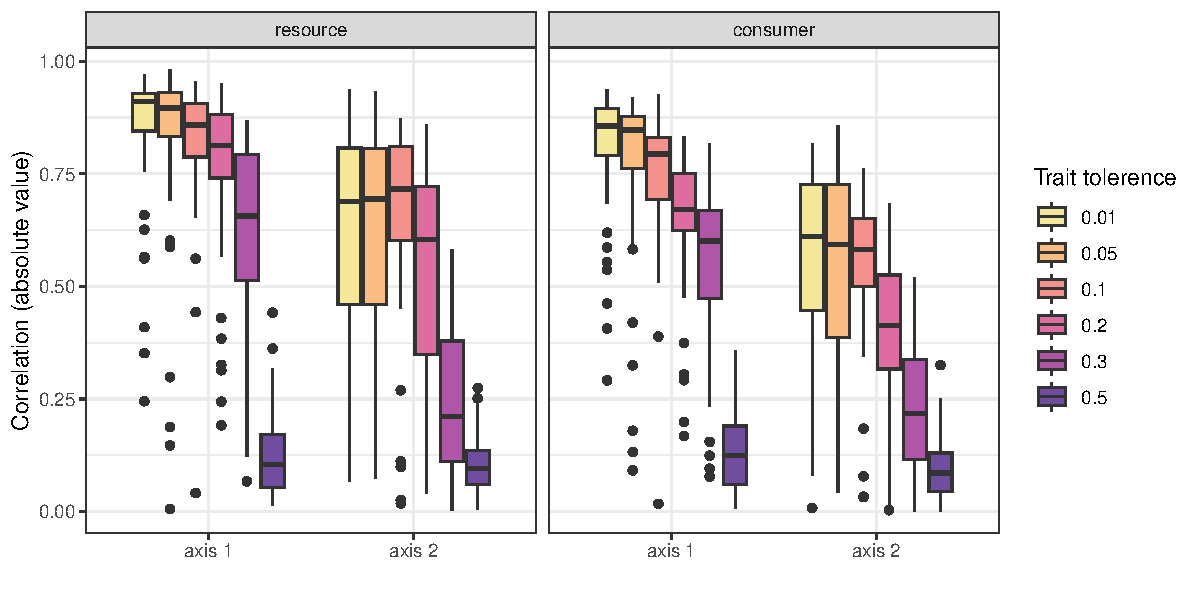
\includegraphics[width=0.75\linewidth]{FIGURES/trait.pdf}
    \caption{Evaluation of the reconstruction of the trait depending on trait tolerance (50 consumer species, 50 resource species, $n_{inter\_tot} = 2500$, $n_{frame} = 5$, $\delta =  0.2$, $trait\_ratio = 0.7$ and $\mu_{tol\_env} = 0.5$)}
    \label{fig:tol_trait}
\end{figure}

The recovery of the traits decreases with increasing trait tolerance ($\mu_{tol\_trait}$). Notably, the trait recovery drastically decreases when $\mu_{tol\_trait}$ exceeds  $0.2$.



%%%%%%%%%%%%%%%%%%%%%%%%%%%



% \subsection{Summary of the Results}

% The impact of the parameters is similar for both consumers and resources. The behavior of the first and second traits is also similar, except for the trait ratio, where the reconstruction of the first trait decreases as the ratio increases, while the second trait's reconstruction improves.

% The number of sampled locations does not significantly change the reconstruction of traits when the environmental tolerance is high (0.5 or greater). However, the reconstruction is more efficient for lower environmental tolerance with either one or many more sampled locations.

% Regarding the weight given to trait matching ($\delta$), a low weight results in poor reconstruction. The reconstruction improves as the weight increases up to 0.2-1 and then decreases.

% Increasing trait tolerance seems to decrease the ability to reconstruct latent traits. However, increasing the sampling effort improves the reconstruction capability.




%%%%%%%%%%%%%%%%%%%%%%%%%%%

Donner les informations sur les param des simu pour chaque légende

raconter une histoire sur pourquoi est ce queue l'on reconstruit le trait matching.

expliquer pourquoi est ce queue il 


%%%%%%%%%%%%%%%%%%%%%%%%%%%

\subsection{Rewiring estimation: correlation of the $\beta$ diversity contribution $\Delta_{OS}$ and the position's variance in the Correspondence Analysis}

\begin{figure}[H]
    \centering
    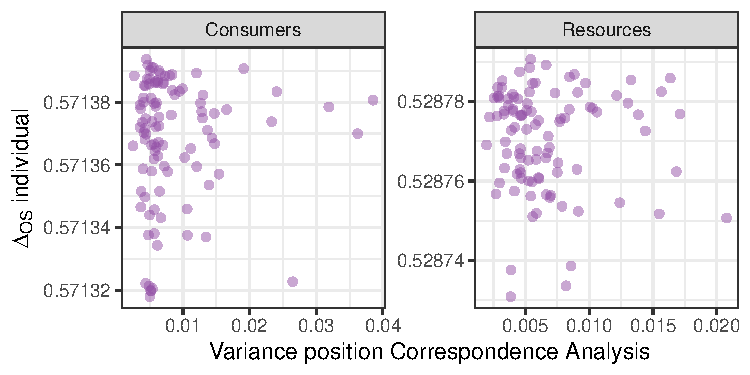
\includegraphics[width=0.75\linewidth]{FIGURES/rewiring.pdf}
    \caption{Comparison of rewiring estimation with the correspondence analysis and with the $\beta$ diversity rewiring contribution (100 consumer species, 100 resource species, $n_{inter\_tot} = 10000$, $n_{frame} = 5$, $\delta =  0.2$, $trait\_ratio = 0.7$, $\mu_{tol\_env} = 0.5$and $\mu_{tol\_trait} = 0.1$)}
    \label{fig:toju}
\end{figure}

There appears to be no correlation between the variance of position in the Correspondence Analysis and the individual contribution to the $\beta$ diversity of link turnover the way it is computed in the article of \citep{toju_interaction_2024}. This lack of correlation is observed for both consumers and resources. The range of the $\Delta_{OS}$ is approximately of order $10^{-5}$ while the variance in position has a range of order $0.02$.



\subsection{Origin of rewiring}

\subsubsection{Environment}

\begin{figure}[H]
    \centering
    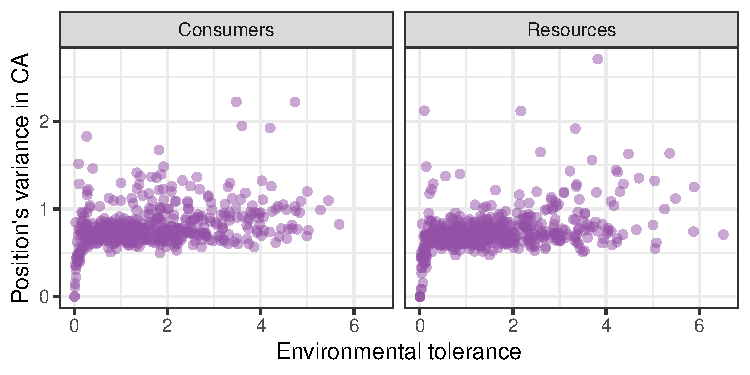
\includegraphics[width=0.75\linewidth]{FIGURES/impact_env.pdf}
    \caption{Effect of the environmental tolerance on the observed position's variance in the CA (500 consumer species, 500 resource species, $n_{inter\_tot} = 25000$, $n_{frame} = 10$, $\delta =  0.2$, $trait\_ratio = 0.7$, $\mu_{tol\_env} = 0.5$ and $\mu_{tol\_trait} = 0.1$)}
    \label{fig:effect_env}
\end{figure}

The position's variance increases when the environmental tolerance ($\mu_{tol\_env}$) is low ($\mu_{tol\_env} < 0.5$), beyond this threshold, the position's variance no longer increases with the environmental tolerance and stabilizes at $1$. 

\subsubsection{Trait}

\begin{figure}[H]
    \centering
    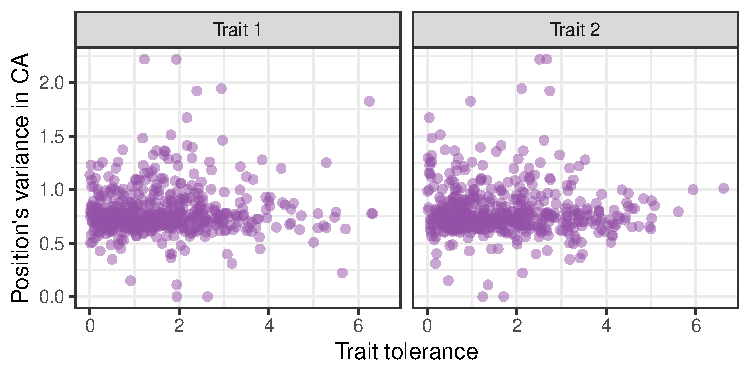
\includegraphics[width=0.75\linewidth]{FIGURES/impact_trait_tol.pdf}
    \caption{Effect of the trait tolerance on the observed position's variance in the CA (500 consumer species, 500 resource species, $n_{inter\_tot} = 25000$, $n_{frame} = 10$, $\delta =  0.2$, $trait\_ratio = 0.7$, $\mu_{tol\_env} = 0.5$ and $\mu_{tol\_trait} = 0.1$)}
    \label{fig:effect_trait}
\end{figure}

There appears to be no significant relationship between trait tolerance ($\mu_{tol\_trait}$)and the variance in the correspondence analysis. The environmental tolerance remains stable at around $0.9$.